This chapter presents an overview of the currently known threat landscape when applying the OAuth protocol. The goal is not only to provide an overview of the threat situation but also to build a base for the decision on which threat category the further experiments of this work focus. Section \ref{sec:oauth_threats} elaborates on every threat separately. The list is mainly based on the current draft for security best practices for OAuth from the OAuth task force at IETF \cite{lodderstedt2020oauth} and is enriched with examples and further explanations.

Section \ref{sec:oauth_countermeasures} showcases different countermeasures, which can be applied to mitigate the presented threats. 

Finally Section \ref{sec:oauth_classification} presents three classifications for the OAuth threats and their countermeasures to aid in giving a practical overview of the OAuth threat landscape and to identify important threat categories.

\section{Threats}
\label{sec:oauth_threats}
Over the 11 years of the existence of OAuth 2.0, there always has been effort dedicated to learning about threats and vulnerabilities, when applying the OAuth 2.0 protocol. When the standard was introduced in 2012 browsers did not have the feature set they provide today, which is important to consider, when analyzing current OAuth threats. Therefore, an elaborate source for getting information about the status of the OAuth threat landscape is the ongoing draft by the OAuth working group of IETF about the best current practice in OAuth security \cite{lodderstedt2020oauth}. As mentioned in Section \ref{subsec:fks_model} the draft is influenced by state-of-the-art research about OAuth security in a collaboration effort. This is the reason this section is mostly based on this draft and enriched with examples of other research work at appropriate places.

Every threat explained in this section receives an encoding in the form of \emph{T<number>} to reference them in later tables. These encodings can be found at the end of the headlines of the following paragraphs.


\subsection[Insufficient Redirect URI Validation]{Insufficient Redirect URI Validation (T1)}
\label{threat:T1}
Insufficient redirect and URI validation poses the risk of adversaries manipulating the redirect flow from the authorization server to the client, to divert the authorization data to an attacker-controlled location. Therefore, authorization servers need to whitelist redirection URLs to make sure, that an attacker cannot craft a hyperlink, which leads to the victim initiating an OAuth flow and sending the authorization code or token to an attacker-controlled domain. Some authorization servers may allow the usage of patterns to allow several domains at once. As well as the absence of any sort of whitelist mechanism even a pattern-matching functionality could lead to security problems. Among the possibility that a user is entering
patterns that are too broad and allow the usage of unintended redirect URLs, the attack surface includes issues with the URL parsing implemented by the authorization server as shown by Wang et al. \cite{wang2019make}. They presented several techniques to trick the parser into accepting unintended domain names, like using squared brackets for IPv6 parsing or the \emph{Evil Slash Trick}, where the parser does not treat a forward slash as a path
separator, while modern browsers do. Depending on the OAuth grant type in use this vulnerability leads to different possibilities to exploit it \cite{lodderstedt2020oauth}.


\subsubsection{Authorization code grant}
Using the example of the authorization code grant the threat of insufficient redirect URI validation can be exploited by crafting arbitrary redirect URIs in the following way:

\begin{enumerate}
    \item The attacker uses techniques like phishing to make its victim open an attacker-controlled webpage, which initiates an OAuth flow with the vulnerable authorization server.
	
    \item The request is crafted with a valid \emph{client ID} (which is public information), the value \emph{code} as response type and a malicious redirect URI, which leads to an attacker-controlled location.
	
    \item If the user logs in at the authorization server, the authorization code now gets transmitted to the attacker's webpage, via the redirect URI query parameter.
	
    \item The attacker can now use the received authorization code, to retrieve a token at the authorization server, if there is no valid session integrity protection over multiple connections in place.
\end{enumerate}


\subsection[Credential Leakage via Referer Headers]{Credential Leakage via Referer Headers (T2)}
\label{threat:T2}
The Referer HTTP header is a potential attack surface. It can be utilized by a
malicious actor to capture query parameters, which are sent via the front-channel, like the state and the authorization code. The authorization code may
be used to redeem an access token before the victim retrieves it and the state
parameter oftentimes includes a CSRF token, which could potentially open up
vulnerabilities in session integrity mechanisms.
\cite{fett2016comprehensive}.

\subsubsection{OAuth Client}
If a client application renders content by an evil third party, like advertisements in iframes or images, before it redeems the authorization code it receives through redirection, an attacker, who places these advertisements or images can potentially capture the code via the referer header of the loaded content and immediately redeem it for an access token.

\subsubsection{Authorization Server}
At the authorization server, \emph{state} query parameters could get leaked via the \emph{Referer} HTTP-header, when third-party images or advertisements are being rendered on the page after the redirection from the client. This may be an issue when the state contains a CSRF token, which as mentioned before could potentially lead to vulnerabilities in session integrity measures.


\subsection[Credential Leakage via History Logs]{Credential Leakage via History Logs (T3)}
\label{threat:T3}
OAuth potentially transports sensitive data via the request-URI, like the access token, as is the case when the implicit grant is used or if other grant types optionally allow the transportation of access tokens or authorization codes via URI parameters. Therefore, a person accessing the user's browser can extract this sensitive data and try to replay it. The same threat is present when a logging server is present, for example, in a corporate network \cite{lodderstedt2020oauth}. Research about browser history security focuses mainly on accessing information about the victim's history by comparing cache timings if a page was visited \cite{bansalcache}. This type of threat is irrelevant in the OAuth context because an attacker would need to guess the access token, which the attacker could endeavor outside the browser history as well. However, recent studies on the security of browser extensions show that malicious browser extensions could access the browser history, or data could be leaked by utilizing vulnerable browser extensions \cite{eriksson2022}. This circumstance more realistically poses a threat to OAuth.

\subsection[Mix-Up Attack]{Mix-Up Attack (T4)}
\label{threat:T4}
In this attack, at least two authorization servers are involved. The target AS and the attacker AS. The OAuth standard allows the resource provider to interact with multiple authorization servers, one of which could be malicious, so the security for such interactions must also be provided. The attack is feasible for the implicit and authorization code grants and works similarly for both. An additional precondition is that the resource owner registers the same redirect URI at both authorization providers, which is typical behavior for Open ID Connect dynamic client registration \cite{hosseyni2023formal}. With these preconditions present, an attacker, which can intercept the victim's requests now waits until the target initializes an OAuth flow with the attacker AS. The attacker then intercepts the initialization request and exchanges the target AS with its attacker AS. When the target client gets redirected to the attacker AS, the target gets immediately redirected back to the target AS for authentication. At the same time, the client ID in the query parameters of the redirection URL gets replaced with the one registered at the target AS. Suppose the target user authenticates because it did not detect that it intended to authenticate at another AS. In that case, an authorization code gets issued to the client when the authorization code grant used. The client then proceeds to try to redeem an access token at the attacker AS, as the client still thinks that it initiated an OAuth flow with the attacker AS. The attacker can now use the received authorization code to redeem an access token at the target AS. \cite{fett2016comprehensive}

\subsection[Authorization Code Injection]{Authorization Code Injection (T5)}
\label{threat:T5} 
The precondition for an authorization code injection is that an attacker has
successfully stolen an authorization code. This can be accomplished in various
ways for example by tricking the user into installing a malicious browser
extension or using other vulnerabilities in a web app like open redirections\cite{philippaerts2022oauch}.

In the case, that the client is using the authorization code grant the attacker can use the stolen authorization code to fetch an access token before the client does.

\subsection[Access Token Injection]{Access Token Injection (T6)}
\label{threat:T6}
This kind of attack describes the process of an attacker using a stolen access token in a legitimate authentication flow, to impersonate the client. If the implicit flow is available, the attacker can now start a new flow and simply replace the access token in the authorization servers' response. This will circumvent any CSRF protection, as there is no difference to a non-compromised
flow. \cite{lodderstedt2020oauth}


\subsection[Cross Site Request Forgery]{Cross Site Request Forgery (T7)}
\label{threat:T7}
This type of attack, often referred to by its abbreviation \emph{CSRF}, is about
the attacker executing a request in the name of the user, by tricking the user
into executing requests for the attacker including all required authentication,
or authorization information. The default OAuth protocol does not include
protection mechanisms against this type of threat. 

\subsection[PKCE Downgrade Attacks]{PKCE Downgrade Attacks (T8)}
\label{threat:T8}
If an authorization server is not implemented to require PKCE for all its
flows, it is susceptible to being vulnerable to PKCE downgrade attacks
\cite{philippaerts2022oauch}. Even if it is documented otherwise, attackers
might try to omit PKCE parameters, as the current OAuth 2.0 standard does not
require the usage of the PKCE extension \cite{hardt2012rfc}. 


\subsection[Access Token Leakage at the Ressource Server]{Access Token Leakage at the Ressource Server (T9)}
\label{threat:T9}
In the scenario that clients can dynamically connect to resource servers at runtime, as is the case in mail or banking applications, an attacker could create a malicious resource server and trick the user into sending valid access tokens for the target data to the malicious resource server, by impersonating a valid resource server. It could also be the case that the client application is misconfigured to send access tokens to a dynamically created resource server. Another vector for access token leakage at the resource server is when the server itself gets compromised, so the attacker receives access tokens by analyzing connections to the server itself \cite{lodderstedt2020oauth}.

\subsection[307 Redirect]{307 Redirect (T10)}
\label{threat:T10}
The OAuth standard does not specify which type of HTTP redirect should be implemented to redirect the user back to the client after the authentication at the authorization server is successful. As the HTTP 307 redirect reuses the header and the body of the original request \cite{fielding1999rfc2616}, a malicious client could extract the username and password of the initial form submission action because it receives this data as part of the redirection \cite{fett2016comprehensive}.

\subsection[Client Impersonating Resource Owner]{Client Impersonating Resource Owner (T11)}
\label{threat:T11}
In the scenario that an authorization server allows for multiple grant types, including the client credentials grant and another typical grant like the authorization code grant, the threat of a malicious client impersonating a resource owner can be present in certain implementations. One example is when the authorization server allows for dynamic registration of clients, with the possibility of setting a client ID. A client could set its ID to the value of an identifying value of a resource owner. To build the example further, Open ID Connect uses a token's subject property to identify a user \cite{sakimura2014openid}. A client could use the subject value as its client ID. Improper implementations of resource servers, which do not distinguish between token types by grant type, could mistake an access token issued to a resource owner with a token issued to a client using the client credentials grant, which allows the malicious client to access the protected data of the resource owner \cite{lodderstedt2020oauth}.


\subsection[Authorization Server Redirecting to Phishing Site]{Authorization Server Redirecting to Phishing Site (T12)}
\label{threat:T12}
When the authorization server allows dynamic client registration, an attacker could create a valid client to which the authorization server could redirect. The attacker then crafts a malicious authorization request that will always fail by appending an invalid \emph{scope} value and then will redirect to the phishing site. An example of such a malicious authorization request is depicted in Figure \ref{fig:phishing_requests}. As the authorization attempt using this crafted URL is always invalid because of the \emph{scope}, the victim immediately gets redirected back to the site given by the \emph{redirect\_uri} parameter, which legally got enlisted through dynamic client registration. This site could be a copy of the valid login page to trick the user into entering its credentials. This way of phishing is very subtle as the domain of the phishing link is valid and known by the victim. The victim would need to identify that the \emph{redirect\_uri} query parameter is invalid and realize that it gets redirected to this URL after clicking on the link with the valid domain \cite{lodderstedt2020oauth}.


\begin{figure}[ht]
	\sffamily\footnotesize
	\url{https://valid-site.com/authorize?scope=invalid&redirect_uri=https://phishing-site.com/login&client_id=client_id_of_malicious_client}
	\special{em:linewidth 0.4pt}
	\linethickness{0.4pt}
	\caption{Phishing request}
	\label{fig:phishing_requests}
\end{figure}

\subsection[Unvalidated Redirects and Forwards]{Unvalidated Redirects and Forwards (T13)}
\label{threat:T13}
This type of vulnerability, known as \emph{Unvalidated Redirects and Forwards} (URF) as well as \emph{Open Redirect}, exists when a web application exposes redirection or forward capabilities to untrusted user input, for example, through query parameters that trigger the redirection. An attacker could generally utilize URF vulnerabilities to craft phishing links that are masked with valid, trustworthy domains \cite{wang2015urfds}. Especially in connection with OAuth, an attacker using an existing URF vulnerability in a client can potentially circumvent whitelists for redirection URIs, by masking the redirect to a malicious client with a valid client exposing an open redirect in the query parameter \cite{lodderstedt2020oauth}. Section \ref{threat:T12} describes a different attack aimed at masking a phishing attack utilizing a mechanism specific to OAuth that is similar to an open redirection at the authorization server and therefore a threat, which is introduced by the implementation of OAuth itself.

\subsection[Clickjacking]{Clickjacking (T14)}
\label{threat:T14}
As authorization servers authorize applications to access confidential data, often through a click of a button, they are susceptible to being targeted by clickjacking attacks. Clickjacking attacks trick users into performing clicks on elements on a web page the users did not intend to interact with, e.g., by overlaying invisible iframes. In the case of OAuth, an attacker could create a malicious application and register it at the authorization server of the target. The attacker also prepares a webpage that tricks the user into clicking on an invisible iframe of the authorization server. The iframe could contain the grant access step of allowing the malicious application to access the user's confidential data. If the user has an active session at the authorization server, a single click is enough to fulfill this action \cite{gibbons2014security}. 


\section{Countermeasures}
\label{sec:oauth_countermeasures}
Addressing the issue of the ever-evolving threat landscape of OAuth several countermeasures have been established in a head-to-head race with the exploitations of vulnerable OAuth implementations. The countermeasures profit from the same circumstance of ongoing browser development as the threats. Countermeasures today can leverage new protection features, which were not present in the past. These countermeasures are also well documented by the OAuth working group of IETF \cite{lodderstedt2020oauth}. In this section, these common countermeasures are briefly explained. Again they receive an encoding at the end of their section's headline for later reference.

\subsection[Mandatory PKCE]{Mandatory PKCE (C1)}
\label{counter:C1}
As an extension to OAuth defined by RFC 7636, \emph{Proof Key for Code Exchange (PKCE)} is a technique to mitigate several OAuth threats \cite{bradley2015rfc}. The main problem PKCE solves for the authorization code grant is verifying that only the original client who started an OAuth flow receives the access token, so a stolen authorization code cannot just get exchanged with an access token by the entity who stole the code. Figure \ref{fig:pkce} shows the way PKCE works \cite{siriwardena_oauth_2020}:

\begin{enumerate}
	\item Initially, before the client redirects the resource owner\'s user agent to the authorization server, it generates a random string of length 43 at minimum, called the \emph{code\_verifier}. It then calculates the hash value of the \emph{code\_verifier} and encodes it with base64 without padding. The hash algorithm in use should be currently regarded as secure and known by the authorization server. The resulting value is called the \emph{code\_challenge}
	
	\item At redirection to the authorization server, the client appends the \emph{code\_challenge} and the hashing algorithm, which it has used to create the \emph{code\_challenge} to the redirection URL as query parameters.
	
	\item After successful authentication, the authorization server creates a record of \emph{code\_challenge} and the corresponding authorization code it generates and redirects the user agent back to the client. Alternatively, it may append the \emph{code\_challenge} to the authorization code and create the record this way.
	
	\item When exchanging the authorization code for an access token, the client sends the \emph{code} and the \emph{code\_verifier} to the authorization server.

	\item The authorization server compares the \emph{code\_verifier} with the corresponding \emph{code\_challenge} of the authorization code by calculating the unpadded base64 encoded hash value of the provided \emph{code\_verifier}. Only the client who initially requested protected resources could possess the random value that matches the \emph{code\_challenge}.
\end{enumerate}


The PKCE mechanism mitigates several threats and vulnerabilities. It mitigates credential leakage via referer headers, as this attack aims in the case of the authorization grant to extract authorization codes after a redirect. Even with a stolen authorization code, an attacker does not know the \emph{code\_verifier} and thus can not receive an access token. For the same reason, any kind of authorization code injection, where the precondition is a stolen authorization code, would only be possible by knowing the \emph{code\_verifier}. Protection against cross-site request forgery is also provided since an attacker could not trick a client into appending confidential data to the resources owned by the attacker, as the victim\'s client does not send the attacker\'s \emph{code\_verifier} to the authorization server. Lastly, protection against PKCE downgrade attacks is ensured when the authorization server implements PKCE as mandatory.

\begin{figure}[H]
	\sffamily\footnotesize
	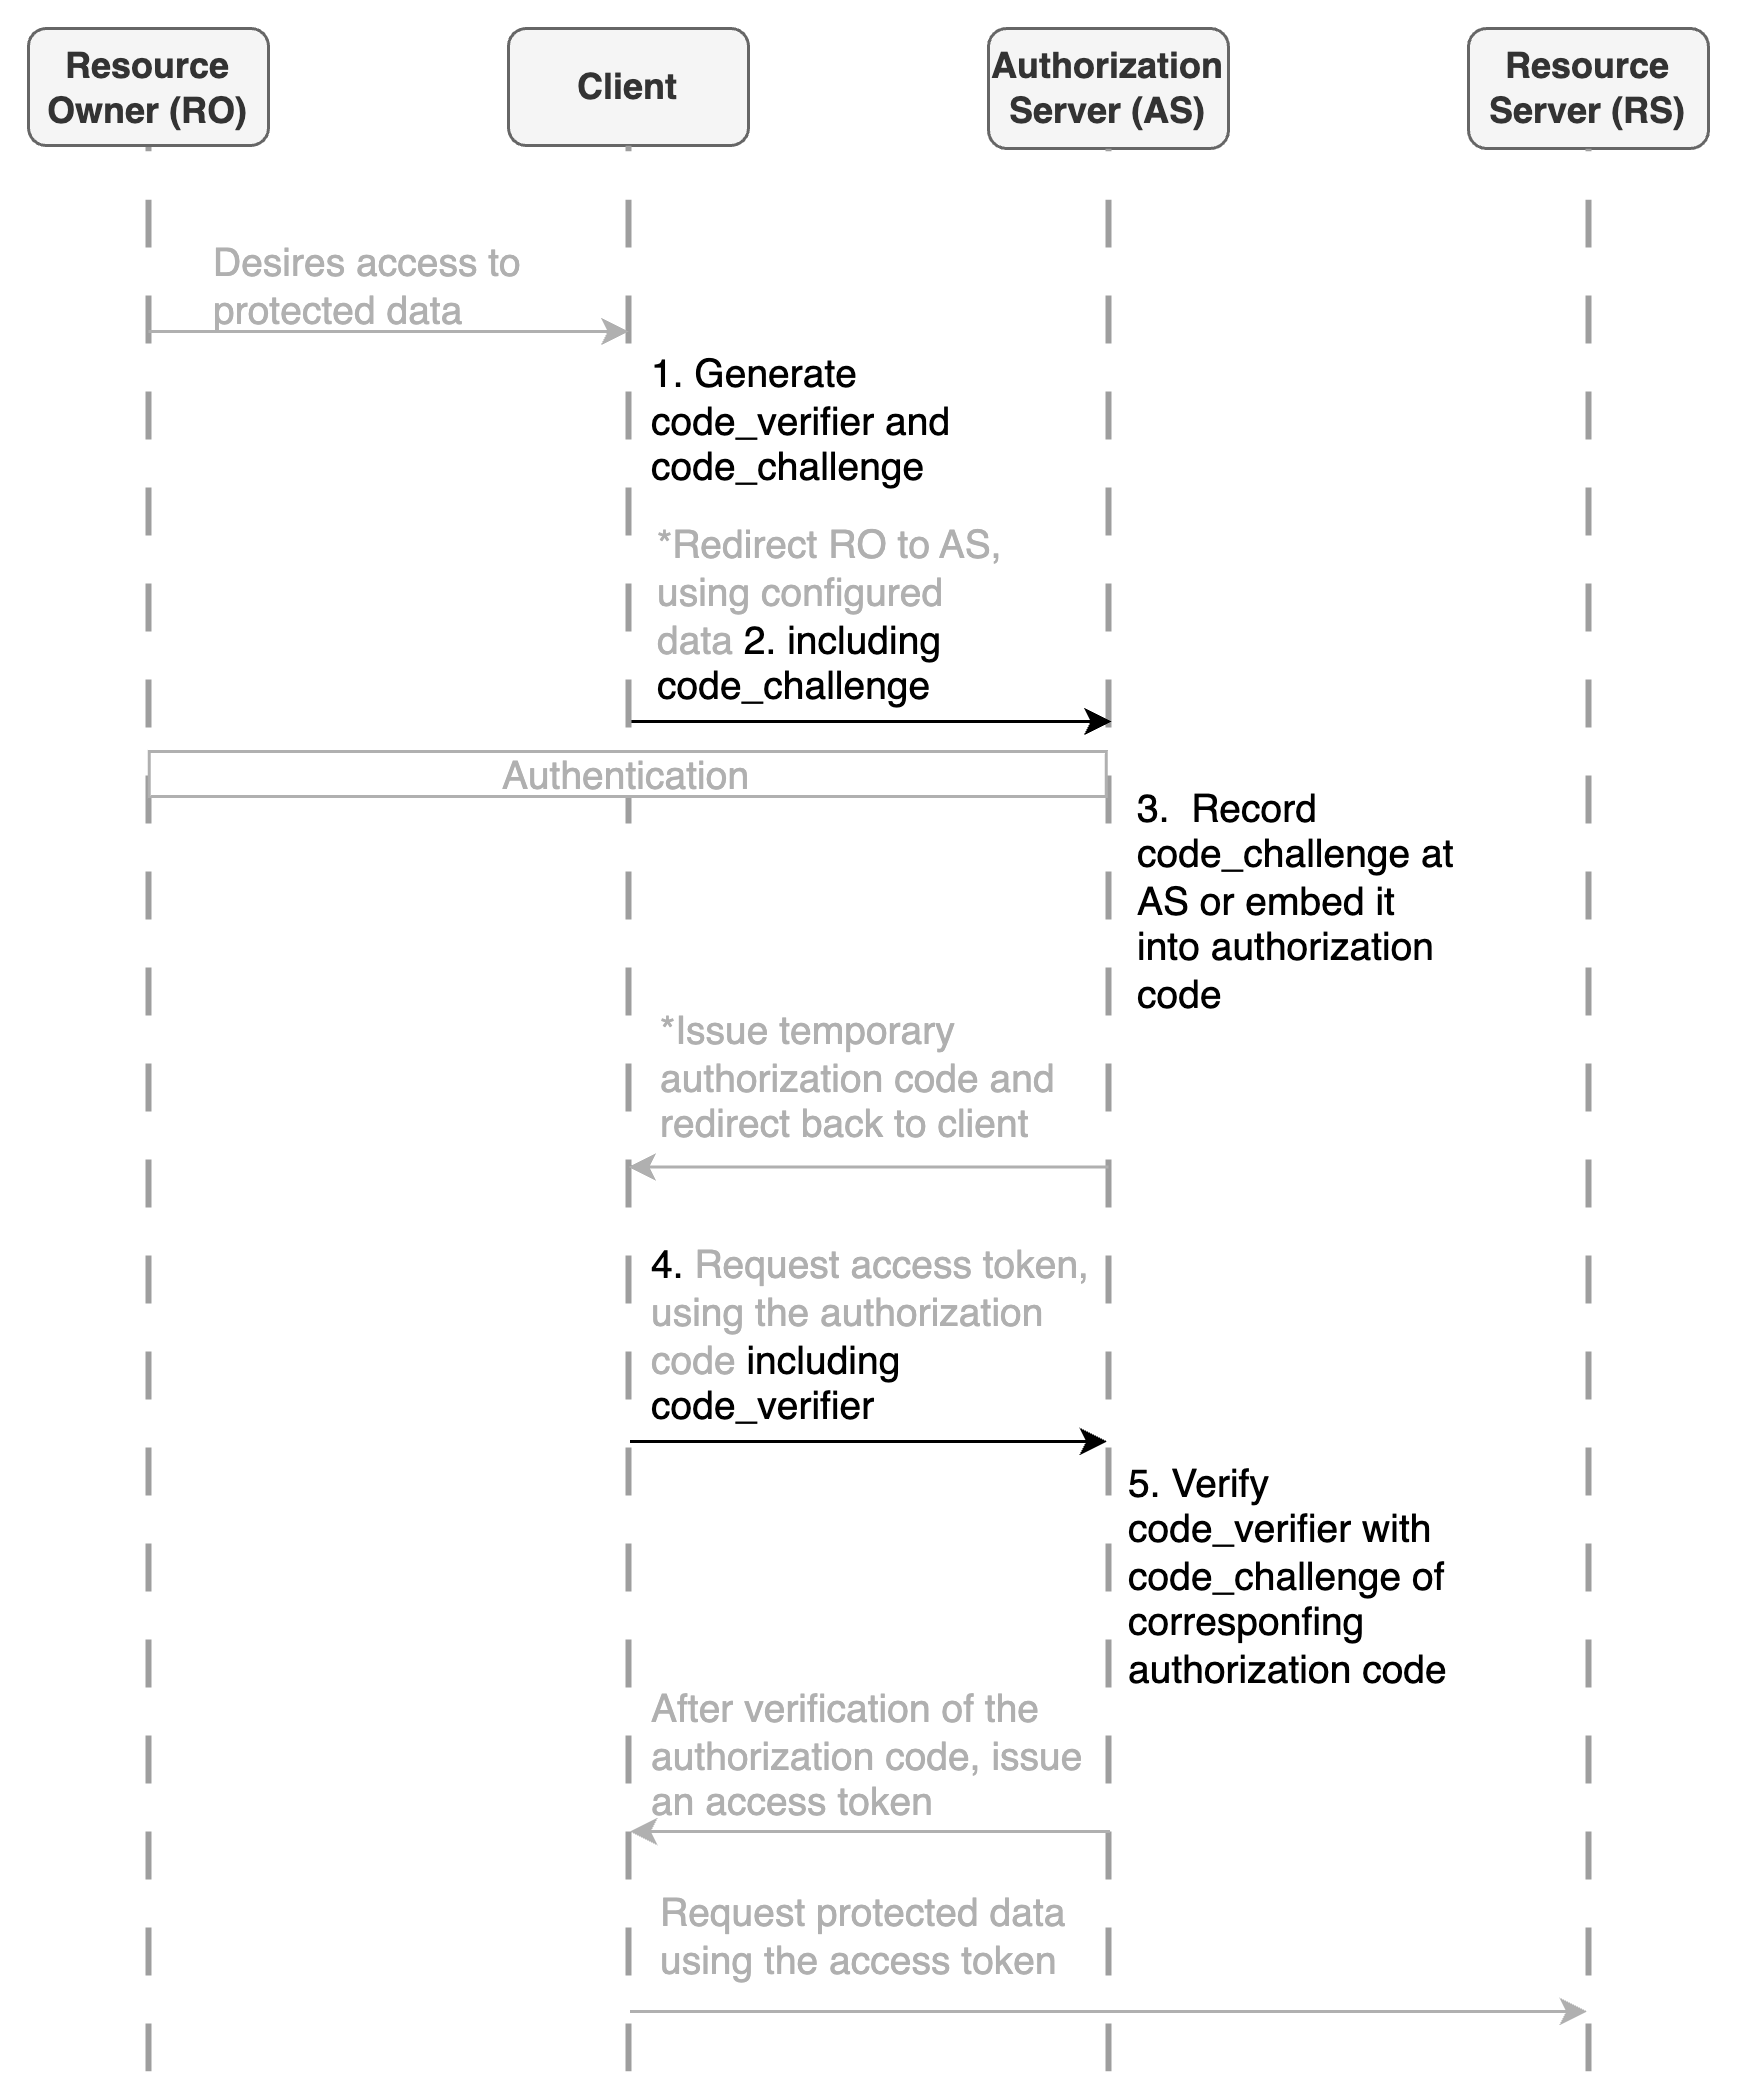
\includegraphics[width=0.75\textwidth]{pic/PKCE.png}
	\unitlength=0.75mm
	\special{em:linewidth 0.4pt}
	\linethickness{0.4pt}
	\caption{Authorization Code Grant with extension for Proof Key for Code Exchange}
	\label{fig:pkce}
\end{figure}

\subsection[Random value state]{Random value state (C2)}
\label{counter:C2}
Another method to protect against Cross-Site request forgery is by taking advantage of the state parameter the OAuth standard offers. When the client initiates an authorization request, it generates a random value of sufficient length, attaches it to the current session and sets it as the state parameter for the request. After authentication, the authorization server has to attach the previously received state parameter to the redirection URI as a query parameter. The client can now validate the received state value with the one it attached to its session earlier to ensure the redirection stems from the authorization flow it initiated \cite{ferry2015security}. When PKCE for the authorization code grant is already implemented, this measure does not add any benefit regarding CSRF protection \cite{bradley2015rfc}. In conclusion, the usages of state's main difference to PKCE is that the client knows that the received authorization code is connected to its initial authorization request before redeeming an access token with the \emph{code\_verifier}, where the authorization server relates the client's requests to each other with the \emph{code\_challenge} and the \emph{code\_verifier}.


\subsection[Invalidation of access tokens]{Invalidation of access tokens (C3)}
\label{counter:C3}
The OAuth framework requires an authorization code to be redeemed only once for an access token. Therefore, an authorization code needs to be invalidated after its first usage. However, this does not stop an attacker from receiving an access token with a stolen authorization code before the valid user does it. The original OAuth 2.0 standard recommends invalidating a previous access token if there was an attempt to receive an access token at least twice for the same authorization code \cite{hardt2012rfc}. Invalidation of access tokens if an authorization code gets redeemed twice helps mitigate the threats of credential leakage via referer headers and credential leakage via browser history \cite{lodderstedt2020oauth}, as for these threats, exposed authorization codes were already redeemed in most cases.

\subsection[Simple string comparision]{Simple string comparision (C4)}
\label{counter:C4}
A technique to completely circumvent the threat of insufficient redirect URI validation is to disallow whitelisting redirect URIs using regular expressions. Instead, exact string comparison is a way to prevent tampering with the redirect URI parameter \cite{lodderstedt2020oauth}.

\subsection[Avoid usage of grant types]{Avoid usage of grant types (C5)}
\label{counter:C5}
Threats like credential leakage via referer headers or browser history can be avoided when the implicit grant is not used at all, as the access token would not be exposed in the URI of a request. Access token injection using the implicit grant makes it easy for any attacker to circumvent CSRF protection through the state parameter (see Section \ref{counter:C2}) since, for the client, it does not make a difference what access token is used for the state check, so an adversary could just start a new implicit grant interaction and inject the token there with a valid state \cite{lodderstedt2020oauth}. For these reasons, the OAuth task force removed the implicit grant in the draft for OAuth 2.1 \cite{hardt2023rfc}. In the past, the main benefit of the implicit grant was that it was possible to implement it for clients that did not utilize cross-origin resource sharing (CORS). CORS was finalized in 2014 by the W3C and superseded by the fetch standard afterward \cite{vanKesteren2014}. As the OAuth standard dates back to 2012 \cite{hardt2012rfc}, the implicit grant could be implemented for applications that did not support CORS yet.

\subsection{Constrained access tokens}
\label{counter:C6_7}
This countermeasure aims to harden the protocol against the misuse of stolen access tokens if they are leaked, for example, at the resource server or through credential leakage via the browser history and or referer headers. It reaches this goal by narrowing the access permissions of the access token in two ways \cite{lodderstedt2020oauth}:
\begin{itemize}
	\item \emph{Sender-constrained access token (C6)}: The token contains cryptographical material to identify the client who redeems the access token, which opens the possibility of only allowing specific clients.
	\item \emph{Audience-constrained access token (C7)}: Access tokens are constrained to particular resource servers. The resource owner executes the audience configuration at the resource server, and the resource server performs the audience verification. If the access token, in addition, bears user-identifying data, different audiences can be defined at the resource server level to further restrain access to the protected data.
\end{itemize}

 
\subsection[Issuer identification]{Issuer identification (C8)}
\label{counter:C8}
Per default, the OAuth authorization grants do not include mechanisms for clients to identify an authorization server, which sends them an authorization response through redirection. This circumstance leads to threats like Mix-Up attacks when multiple authorization servers are involved. Issuer identification has been introduced to tackle this issue with RFC9207 in 2022. The issuer identifier \emph {iss} is a parameter that must be sent to the client in every response, even if it is an error response. The \emph{iss} parameter contains the URL, which points to the metadata of the authorization server. This metadata has to include an \emph{issuer} property, which contains a value identical to the value of the \emph{iss} property. The client, which supports issuer identification, has to store the identifier locally when initiating an interaction with an authorization server. The client then must compare the stored value with the one it receives from the authorization response with a simple string comparison. The client is also responsible for ensuring that every authorization server it interacts with holds a unique issuer identifier \cite{meyer2022rfc}.


\subsection{Implementation details}
\label{counter:C9_10_11_12_13_14}

There are several countermeasures that one can categorize as implementation details, as they are applied through small decisions during client or authorization server implementation. The following is a brief list of these measures and the classification of which involved party is responsible for implementing the measure.
\begin{itemize}

\item \emph{303 redirect (C9)}: As mentioned in Section \ref{threat:T10}, the OAuth standard does not mandate the type of HTTP redirect to use for authorization servers. To circumvent issues with improper redirect handling leading to security issues, the authorization server should use 303 redirects.

\item \emph{Client\_ID not choosable by user (C10)}: To mitigate threats that arise through the possibility of a client choosing its own client ID, as described in Section \ref{threat:T11}, the client ID should always be chosen at random by the authorization server, where the clients are getting registered.

\item \emph{No redirect before authentication at authorization provider (C11)}: Some threats arise because authorization servers might be implemented in a way that they are redirecting the user agent in error cases, even without complying with the redirect URI whitelists in some cases. This behavior could lead to advanced phishing attacks as described in Section \ref{threat:T4}. Therefore, authorization servers should be implemented in a way that they only redirect the user agent if the authentication of the resource owner has been successful.

\item \emph{No access token in URI (C12)}: The OAuth standard allows for access tokens to be transported in the request URI from the client to the authorization server when accessing protected data, even when the authorization code grant is in use. This option leads to threats concerning leakage of the access token through browser history or referer headers. Therefore, an authorization server should implement the transporting of the access token through a request body as mandatory.

\item \emph{Avoid third-party content on pages involved with OAuth (C13)}:
\label{item:avoid3rd}
Malicious advertisements in iframes or attacker-generated hyperlinks on pages an OAuth flow redirects to could lead to leakage of access tokens or authorization codes through referer headers. Therefore, authorization servers and clients must ensure that no third-party content is allowed for the redirection endpoint at the client and authentication page at the authorization server.

\item \emph{Appropriate Referer Policy (C14)}: On top of the measure described above about rendering of third-party content, to mitigate credential leakage via referer headers, an appropriate referer header policy should be implemented like the \emph{Referrer-Policy: no-referrer} header in authorization requests or as a meta tag in HTML documents.

\end{itemize}

\subsection{General web security countermeasures}
\label{counter:C15_16}
After laying out several mitigations for attack vectors of OAuth, there are still general web security threats, which are especially important for OAuth, like clickjacking or open redirections. The reason why these common web security vulnerabilities are critical in the case of OAuth has been laid out in their specific sections. The countermeasures for those types of vulnerabilities, however, are very context-specific and are out of the scope of this work. Hence, in further portrayals of threats and countermeasures in this work, they are described as countermeasures against clickjacking (C16), and open redirect (C15), but do not include specifics.

\section{Classification of OAuth threats and vulnerabilities}
\label{sec:oauth_classification}
After laying out the threats and their respecting countermeasures, it is evident that the OAuth authorization framework tries to solve a lot of practical authorization use cases at once which leads to different threats in different situations, requiring adequate countermeasures. To form a general, even more tangible overview of the threat situation of OAuth, this work proceeds to provide different perspectives on the threat landscape, as well as a broad categorization of similar threat types.

\subsection{Threats and their countermeasures}

The first classification displayed in Table \ref{tab:txc} is visualizing, which countermeasure mitigates aspects of which threat when using OAuth. The table shows that most countermeasures are specific to single threats. However, there are two countermeasures, which mitigate at least three threats. These countermeasures are mandatory PKCE and avoiding the usage of specific grant types. Looking at the problems these two countermeasures solve, one can identify the two main weaknesses of the OAuth 2.0 standard. The first one being grant types like the implicit grant, which communicate confidential messages via the front-channel. The second weakness being the session integrity of the protocol, as multiple connections are involved via redirections. Both these countermeasures will be enforced by the OAuth 2.1 standard \cite{hardt2023rfc}, which makes conforming implementations potentially a lot more secure in the future.

\begin{table}[H]
	\caption{Classification of which countermeasure mitigates which threat to OAuth. \emph{The encoding T1-T14 corresponds to the threats described in Section \ref{sec:oauth_threats}}.}
	\label{tab:txc}
	\begin{tabular}{|c|c|c|c|c|c|c|c|c|c|c|c|c|c|c|c|c|}
	\hline
	 & \rot{\hyperref[counter:C1]{\textbf{Mandatory PKCE}}} & \rot{\hyperref[counter:C2]{\textbf{Random value state}}} & \rot{\hyperref[counter:C3]{\textbf{Invalidation of access tokens}}} & \rot{\hyperref[counter:C4]{\textbf{Simple string comparision}}} & \rot{\hyperref[counter:C5]{\textbf{Avoid usage of grant types}}} & \rot{\hyperref[counter:C6_7]{\textbf{Sender-constrained access token}}} & \rot{\hyperref[counter:C6_7]{\textbf{Audience-constrained access token}}} & \rot{\hyperref[counter:C8]{\textbf{Issuer identification}}} & \rot{\hyperref[counter:C9_10_11_12_13_14]{\textbf{303 redirect}}} & \rot{\hyperref[counter:C9_10_11_12_13_14]{\textbf{Client\_ID not choosable by user}}} & \rot{\hyperref[counter:C9_10_11_12_13_14]{\textbf{No redirect before authentication at AS }}} & \rot{\hyperref[counter:C9_10_11_12_13_14]{\textbf{No access token in URI}}} & \rot{\hyperref[counter:C9_10_11_12_13_14]{\textbf{Avoid third-party content}}} & \rot{\hyperref[counter:C9_10_11_12_13_14]{\textbf{Appropriate referer policy}}} & \rot{\hyperref[counter:C15_16]{\textbf{Open redirect countermeasure}}} & \rot{\hyperref[counter:C15_16]{\textbf{Clickjacking countermeasure}}} \\ \hline
	\hyperref[threat:T1]{\textbf{T1}}             &             &             &             & x           &             &    &    &    &    &     &     &     &     &     & x   &     \\ \hline
	\hyperref[threat:T2]{\textbf{T2}}              & x           &             & x           &             & x           &    &    &    &    &     &     &     & x   & x   &     &     \\ \hline
	\hyperref[threat:T3]{\textbf{T3}}              &             &             & x           &             & x           &    &    &    &    &     &     & x   &     &     &     &     \\ \hline
	\hyperref[threat:T4]{\textbf{T4}}              &             &             &             &             &             &    &    & x  &    &     &     &     &     &     &     &     \\ \hline
	\hyperref[threat:T5]{\textbf{T5}}              & x           & x           &             &             &             &    &    &    &    &     &     &     &     &     &     &     \\ \hline
	\hyperref[threat:T6]{\textbf{T6}}              &             &             &             &             & x           &    &    &    &    &     &     &     &     &     &     &     \\ \hline
	\hyperref[threat:T7]{\textbf{T7}}              & x           & x           &             &             &             &    &    &    &    &     &     &     &     &     &     &     \\ \hline
	\hyperref[threat:T8]{\textbf{T8}}              & x           &             &             &             &             &    &    &    &    &     &     &     &     &     &     &     \\ \hline
	\hyperref[threat:T9]{\textbf{T9}}              &             &             &             &             &             & x  & x  &    &    &     &     &     &     &     &     &     \\ \hline
	\hyperref[threat:T10]{\textbf{T10}}             &             &             &             &             &             &    &    &    & x  &     &     &     &     &     &     &     \\ \hline
	\hyperref[threat:T11]{\textbf{T11}}             &             &             &             &             &             &    &    &    &    & x   &     &     &     &     &     &     \\ \hline
	\hyperref[threat:T12]{\textbf{T12}}             &             &             &             &             &             &    &    &    &    &     & x   &     &     &     &     &     \\ \hline
	\hyperref[threat:T13]{\textbf{T13}}             &             &             &             &             &             &    &    &    &    &     &     &     &     &     & x   &     \\ \hline
	\hyperref[threat:T14]{\textbf{T14}}             &             &             &             &             &             &    &    &    &    &     &     &     &     &     &     & x   \\ \hline
	\end{tabular}
	\end{table}

\subsection{Threats by mitigation responsibility}
Another way to put the threat landscape into perspective is by categorizing the different threats by the entities, which are responsible for mitigation. Depicted in Table \ref{tab:mitigation_responsibility} it is visible, that most threats need to be mitigated by the client and the authorization server together. This is not surprising as one goal of OAuth is to provide a modular authorization workflow, so the resource server for example only needs to provide a token verification ability for the protocol. Important to note is that most countermeasures are enforced by the authorization server as the client is more or less a consumer of the authorization service. If an authorization server decides to enforce countermeasures like PKCE (\hyperref[counter:C1]{C1}) a client has to adapt to this requirement. Therefore even if many of the countermeasures need to be realized by the client and authorization server together, in practice the authorization server bears the main responsibility for fulfilling mitigation efforts. An additional aspect of the table to consider is that there are still threat aspects, that only the client can handle. General web security threats like unvalidated redirects and forwards (open redirects) and clickjacking are threats that could be chained together with other OAuth threats for exploitation. These are examples of dangers the authorization server cannot influence.

\begin{table}[H]
	\caption{Classification of threats by mitigation responsibility. \emph{The encoding C1-C16 corresponds to the countermeasures described in Section \ref{sec:oauth_countermeasures}}.}
	\label{tab:mitigation_responsibility}
	\begin{tabular}{|l|l|l|l|}
	\hline
	\textbf{Threat}                                                                                       & \textit{Client}                                                 & \textit{Authorization Server}                                                 & \textit{Resource Server} \\ \hline
	\textit{Insufficient Redirect URI Validation}                                                         &                                                                 & C4                                                                            &                          \\ \hline
	\textit{\begin{tabular}[c]{@{}l@{}}Credential Leakage via \\ Referer Headers\end{tabular}}            & \begin{tabular}[c]{@{}l@{}}C1, C5, C12,\\ C13, C14\end{tabular} & \begin{tabular}[c]{@{}l@{}}C1, C3, C5,\\ C6, C7, C12,\\ C13, C14\end{tabular} &                          \\ \hline
	\textit{\begin{tabular}[c]{@{}l@{}}Credential Leakage via \\ History Logs\end{tabular}}               & C5, C12                                                         & C3, C5, C12                                                                   &                          \\ \hline
	\textit{Mix-Up Attacks}                                                                               & C8                                                              & C8                                                                            &                          \\ \hline
	\textit{Authorization Code Injection}                                                                 & C1                                                              & C1, C3                                                                        &                          \\ \hline
	\textit{Access Token Injection}                                                                       & C5                                                              & C5                                                                            &                          \\ \hline
	\textit{Cross-site Request Forgery}                                                                   & C1, C2                                                          & C1, C2                                                                        &                          \\ \hline
	\textit{PKCE Downgrade Attacks}                                                                       & C1                                                              & C1                                                                            &                          \\ \hline
	\textit{\begin{tabular}[c]{@{}l@{}}Access Token Leakage \\ at the Ressource Server\end{tabular}}      & C6, C7                                                          & C6, C7                                                                        & C6, C7                   \\ \hline
	\textit{307 Redirect}                                                                                 &                                                                 & C9                                                                            &                          \\ \hline
	\textit{Client impersonating resource owner}                                                          &                                                                 & C10                                                                           &                          \\ \hline
	\textit{\begin{tabular}[c]{@{}l@{}}Authorization Server \\ Redirecting to Phishing Site\end{tabular}} &                                                                 & C11                                                                           &                          \\ \hline
	\textit{Unvalidated Redirects and Forwards}                                                           & C15                                                             &                                                                               &                          \\ \hline
	\textit{Clickjacking}                                                                                 & C16                                                             & C16                                                                           &                          \\ \hline
	\end{tabular}
	\end{table}

\subsection{Threats by properties in common}
Another way for classification proposed by this work is to sort the different threats by common properties to determine threat categories and possibly identify more impactful groups of threats. One possible categorization is portrayed in Figure \ref{fig:threat_taxonomy}:
\begin{enumerate}
	\item \emph{Credential leakage and session hijacking}: Threats . that have in common that through different web technologies, like HTTP, HTML, and browser features such as history logs and certain implementation flaws, the credentials of a user, or an active session could get leaked to an adversary. These threats must be mitigated by different mechanisms these web technologies offer, like strict content security policies, adequate referer header policies and measures that prevent the use of stolen authorization codes and access tokens. 
	\item \emph{Redirection tampering}: Threats that are characterized by the possibility that an adversary tampers with the redirection flow of an OAuth grant. These threats are often bound to flaws in the implementation of OAuth by the client and the authorization server, combined with phishing. These threats are among the most impactful threats as they allow for an attacker to completely impersonate the victim, by just crafting a malicious URL and making the victim click on it and potentially persisting session integrity.
	\item \emph{Breaking of protocol integrity}: Threats for mechanisms to ensure session integrity like CSRF tokens in the state parameter or PKCE. These measures could have a flawed implementation or could be optional leading to the possibility an adversary could circumvent them.
	\item \emph{Credential Injection}: If credentials are already leaked, one category of threats is the threat of the injection of these credentials into the protocol. Certain measures can be introduced to even mitigate the injection at this point, by one-time tokens connected with invalidation of used tokens, or short timespans for redeeming access tokens for authorization codes.
\end{enumerate}

\begin{figure}[H]
	\sffamily\footnotesize
	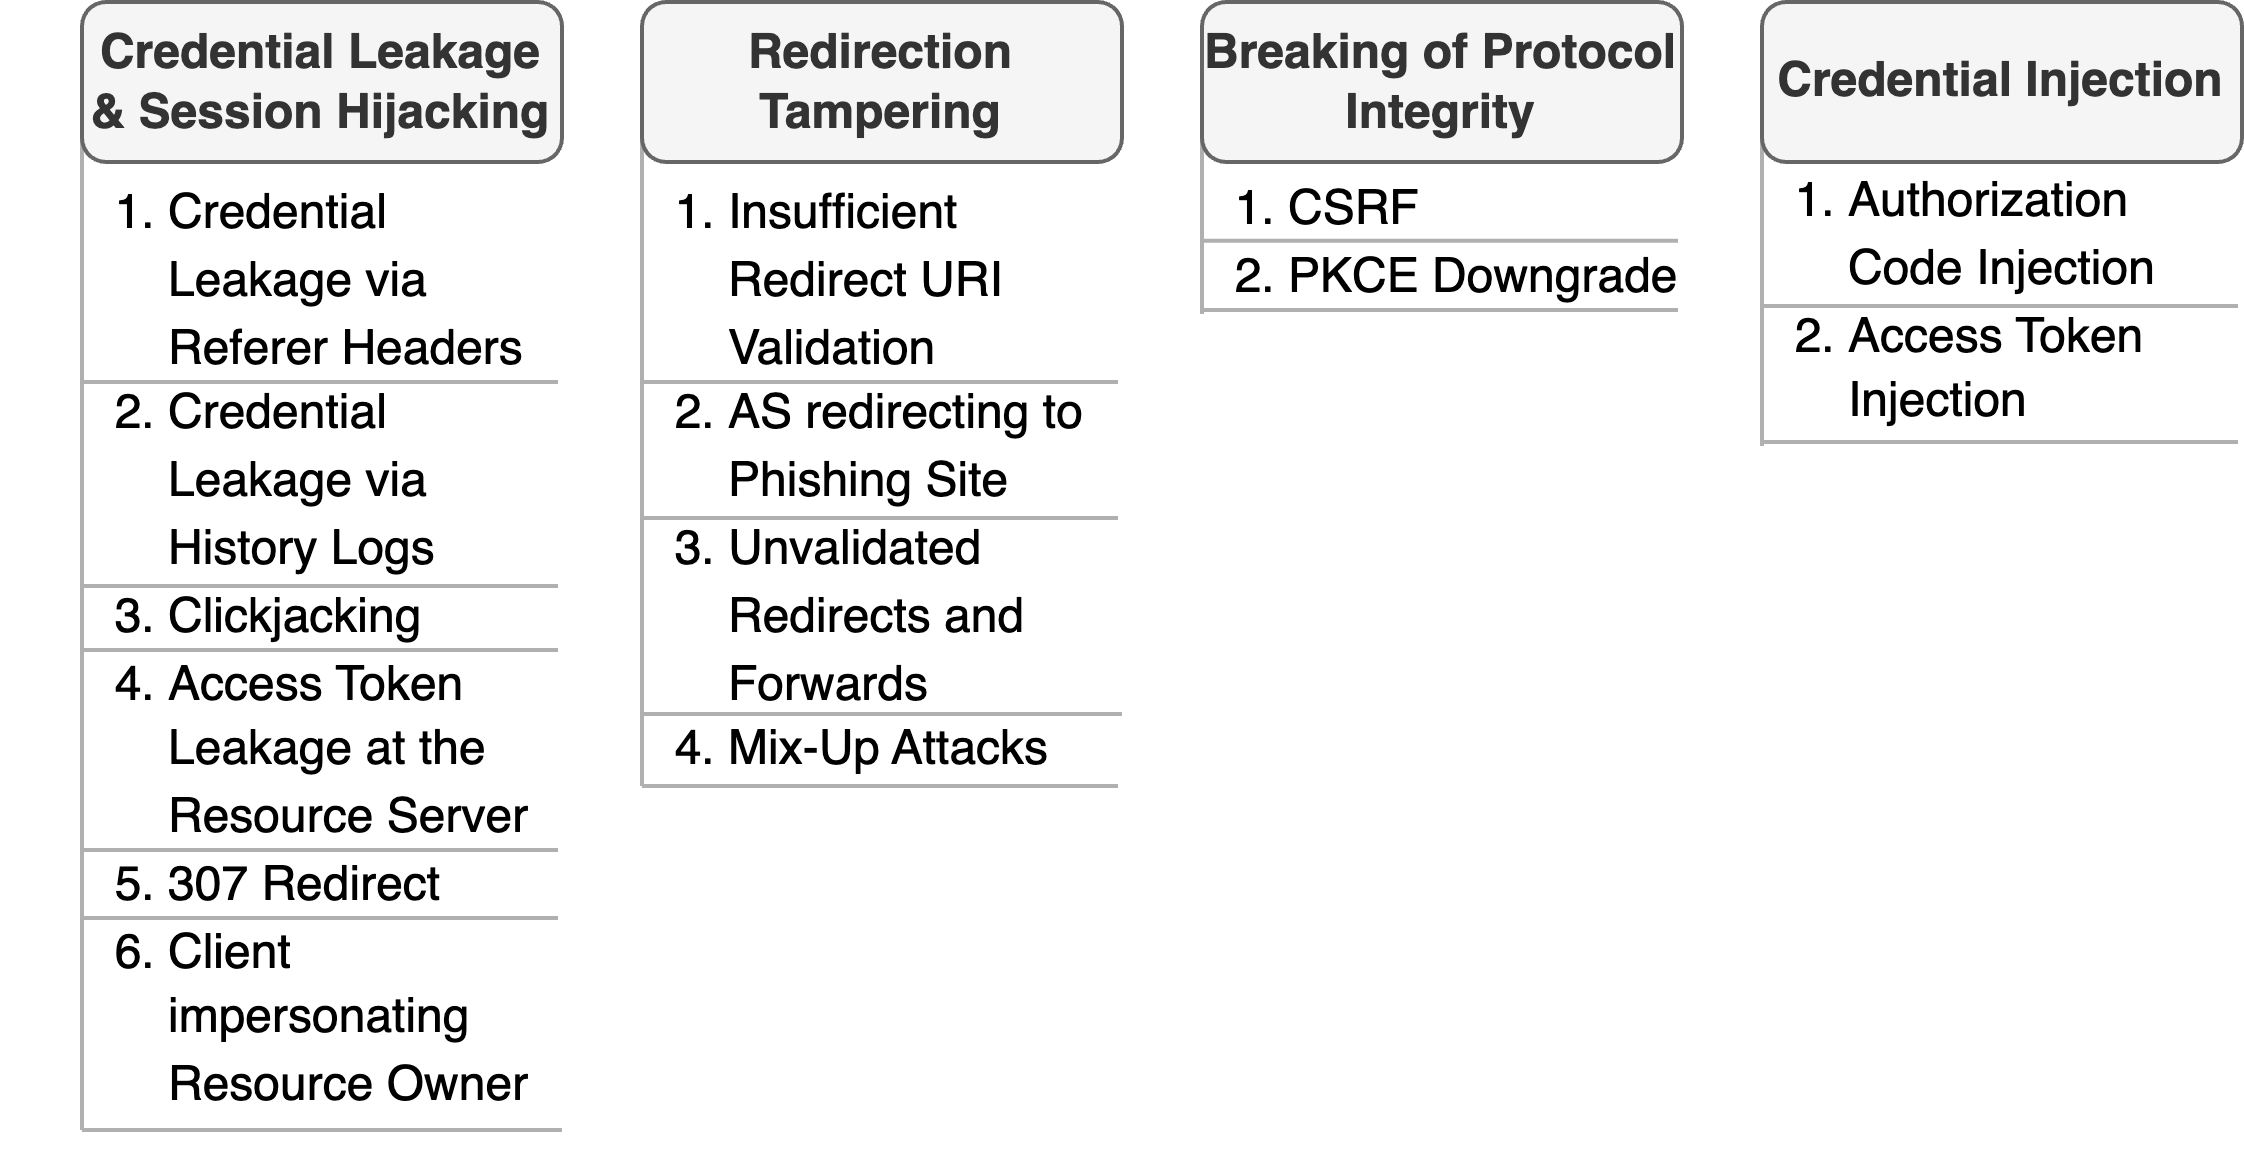
\includegraphics[width=1\textwidth]{pic/threat_taxonomy.png}
	\unitlength=0.75mm
	\special{em:linewidth 0.4pt}
	\linethickness{0.4pt}
	\caption{Threats categorized by properties in common}
	\label{fig:threat_taxonomy}
\end{figure}

Following along with this categorization, the \emph{Redirection Tampering} category was chosen for further analysis in the intrusion detection experiment of this work, as the potential vulnerabilities that are involved with this threat category are more directly tied to flaws in OAuth implementations instead of problems which arise through other web technologies. In addition, these threats are potentially highly impactful with comparable low effort from the adversary (except for the Mix-Up attacks), if a vulnerability is present.